\section{Evaluation}
\label{sec:validation}

The evaluation of our approach is twofold. First, we evaluate \textit{correctness}. To this end, we use a test oracle consisting of a well-documented case study where we exactly know the existing overlapping among the involved DSLs. We execute our approach on the case study and we check that the input matches the expected overlapping. Second, we evaluate \textit{relevance}. More concretely, we use empirical data to demonstrate that the phenomenon of syntactic and semantic overlapping is actually appearing in realistic DSLs that we obtain from public \texttt{GitHub} repositories. Thus, we show that there is room in real projects to the applicability of our approach.  

\textbf{Implementation and hardware used $\rightarrow$} The approach presented within this paper is implemented in the puzzle toolsuite~\footnote{\url{puzzle.github.io}}. Puzzle have been developed as an Eclipse-based~\footnote{eclipse} language workbench. Metamodels are specified in the Ecore language whereas domain-specific actions are specified as methods in Xtend programming language~\footnote{\url{http://www.eclipse.org/xtend/}}. The mapping between metaclasses and domain-specific actions is specified by using the notion of aspect introduced by the Kermeta 3~\footnote{\url{https://github.com/diverse-project/k3/wiki/Defining-aspects-in-Kermeta-3}} that realize the ideas presented in \cite{}. \todo{cita tambien a melange si procede.}

\todo[inline]{podriamos comentar al final esto ya que no reportamos en tiempo... pero mejor tener los datos}
For the first experiment, Puzzle was executed in a Pc running MacOs X with XX Gb of ram and with a XXX Intel CPU. Then, for the second, a custom version of puzzle was extracted as an executable jar and executed within Grid5000~\url{https://www.grid5000.fr} to distribute the workload of analyzing all the possible overlaping within more than 2000 models. Concretely we used 1000 Intel Xeon CPUs at 2100Ghz available in the Nancy cluster.  

\subsection{Experiment 1: Evaluating \textit{correctness} with the state machines case study}

The case study we use to evaluate the correctness of our approach was introduced by Crane et al \cite{Crane:2007}, and it is composed of three different DSLs for expressing state machines: UML state diagrams, Rhapsody, and Harel's state charts. This case study describes a realistic problematic that has an impact on the industry. As a matter of fact, it is one of the motivations of the VaryMDE\footnote{\url{http://varymde.gforge.inria.fr/}} project which is a collaboration between Thales Research \& Technology, and INRIA.

\vspace{-3mm}
\subsubsection{The test oracle:} Naturally, because the three DSLs are intended to express the same formalism, they have commonalities, namely, overlapping. For example, all of them provide basic concepts such as \texttt{StateMachine}, \texttt{State}, \texttt{Transition}, or \texttt{Trigger}. However, not all those DSLs are exactly equal. They have both syntactic and semantic differences which are well documented in the Crane's article \cite{Crane:2007}.

Syntactic differences are materialized by the fact that not all the DSLs provide exactly the same constructs. Figure \ref{fig:oracle} shows a table with the language constructs provided by each DSL. There are differences in the support for transition's triggers and pseudostates. Whereas Rhapsody only supports simple triggers. Harel's state charts and UML provide support composed triggers. More concretely, in Harel's state charts triggers can be composed by using \texttt{AND}, \texttt{OR}, and \texttt{NOT} operators. In turn, in UML triggers can be composed by using  the \texttt{AND} operator.

In addition, whereas there are pseudostates that are supported by all the DSLs (\texttt{Fork}, \texttt{Join}, \texttt{ShallowHistory}, and \texttt{Junction}); there are two psueudostates i.e., \texttt{DeepHistory} and \texttt{Choice} that are only supported by UML. The \texttt{Conditional} pseudostate is only provided by Harel's state charts.

In summary, there are: \textbf{17} language constructs that are shared by all the DSLs; \textbf{1} construct that is exclusive of UML; \textbf{2} constructs that are exclusive of Harel's state charts; \textbf{2} constructs shared by UML and Harel's state charts; and, finally, \textbf{1} construct shared by Harel's state charts and Rhapsody. 

\begin{figure}
\centering
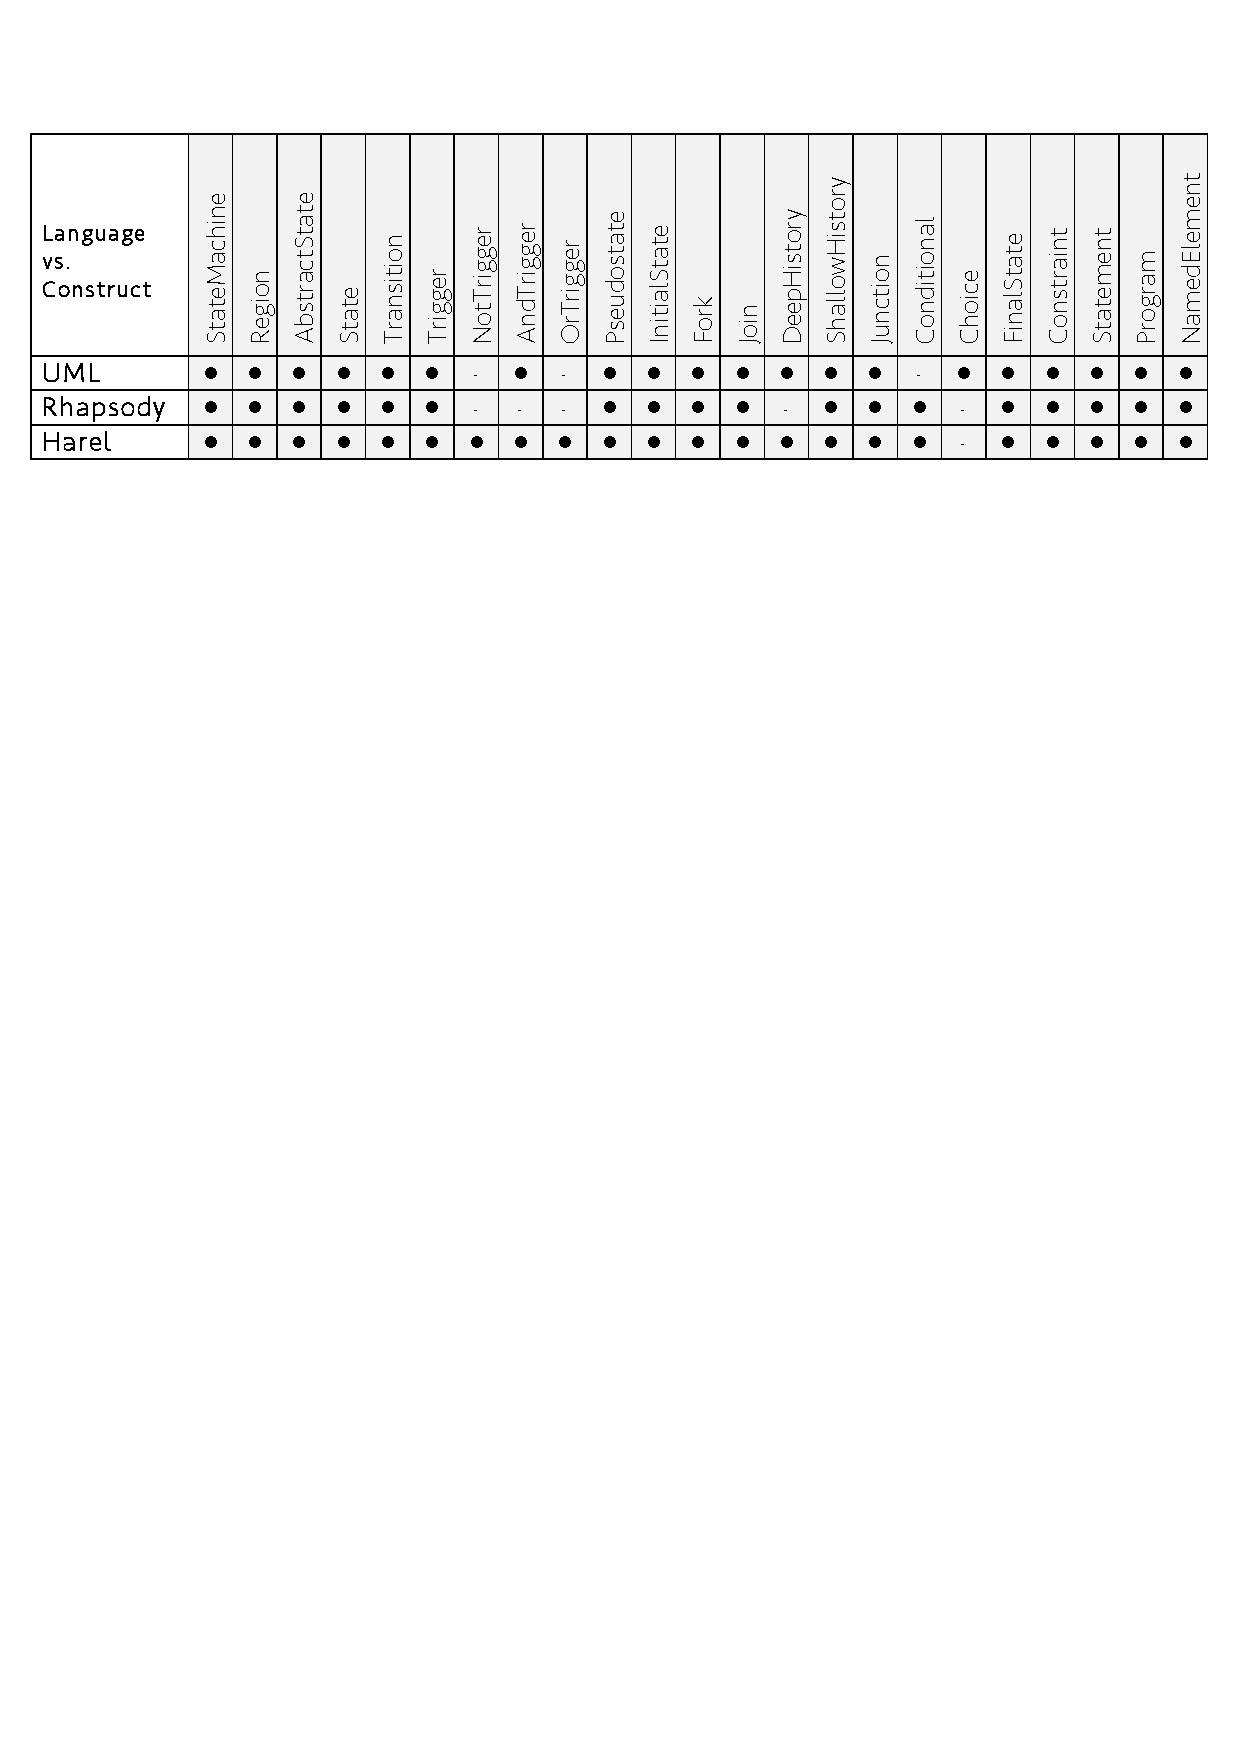
\includegraphics[width=1\linewidth]{images/oracle.pdf}
\caption{Oracle for evaluation of correctness}
\label{fig:oracle}
\end{figure}

Semantic differences are materialized by the fact that not all the DSLs have the same behavior at execution time. For example, whereas in Harel's state charts simultaneous events are attended in parallel, both UML and Rhapsody follow the run to completion principle so simultaneous events are attended sequentially. 

As a direct consequence of those semantic differences, not all the domain-specific actions are the same. For instance, due to the semantic difference in the events treatment policy explained above, the methods \texttt{eval()} and \texttt{step()} in the \texttt{StateMachine} metaclass are different in each DSL. 

\vspace{-3mm}
\subsubsection{Results:} Let us now analyze the results we obtained from the execution of our approach on the test oracle. Figure \ref{fig:puzzle-overlapping} shows the results of the first part of the analysis. It presents the Venn diagram that shows syntactic and semantic overlapping. Note that, in the case of the syntactic overlapping, the cardinalities of the intersections in the Venn diagram match the test oracle thus, demonstrating that our approach to comparison of metaclasses is correct. In turn, the methods \texttt{eval()} and \texttt{step()} of the \texttt{StateMachine} metaclass are correctly identified as different in each DSL.

\begin{figure}
\centering
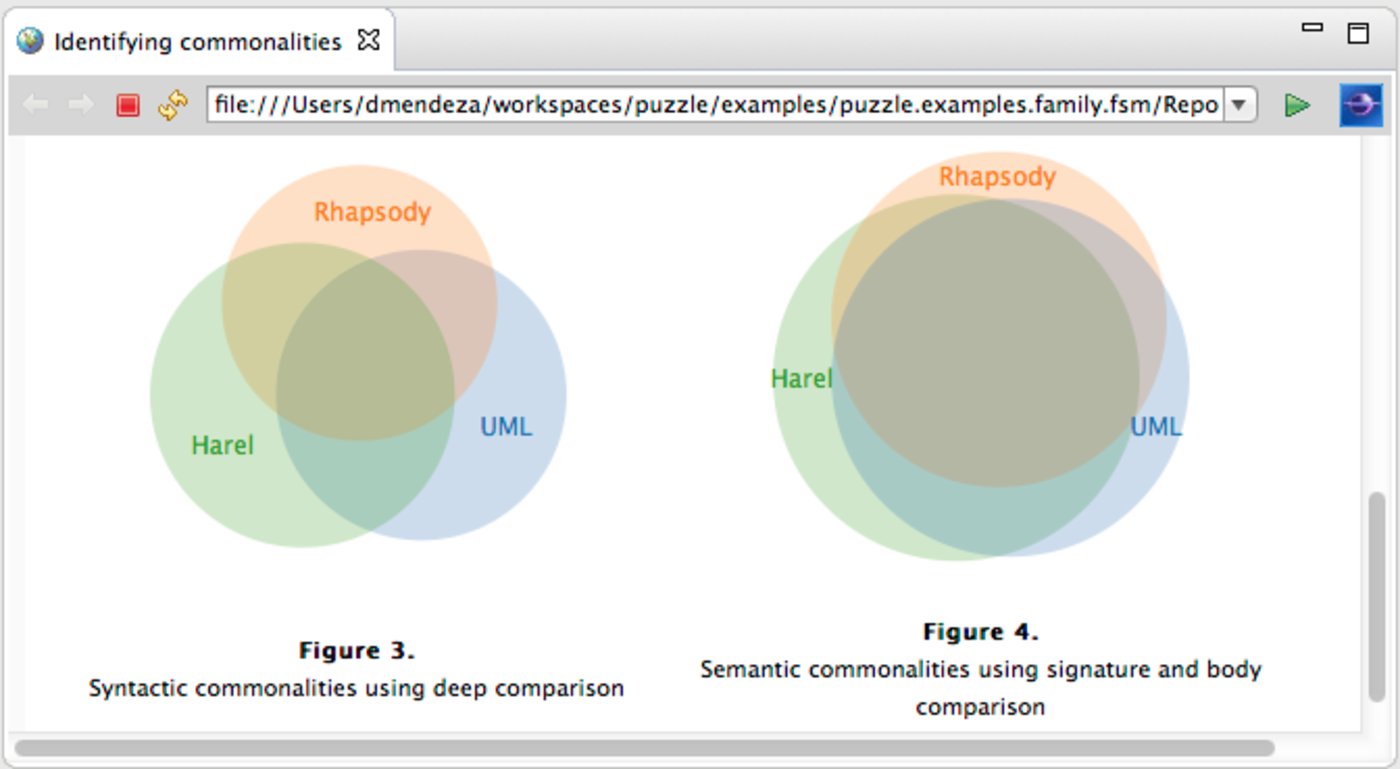
\includegraphics[draft,width=1\linewidth]{images/puzzle-overlapping.pdf}
\caption{Overlapping detected using the Puzzle toolsuite in the state machines case study. }
\label{fig:puzzle-overlapping}
\end{figure}

Figure \ref{fig:puzzle-modularization} shows the results for the second and third steps of our approach: identifying and extracting reusable language modules. There is a language module that contains all the language constructs shared by the three DSLs. This language module can be considered as a basic DSL for state machines that supports the basic constructs. It can be used in the construction of new DSLs for state machines. In addition, there are other language modules encapsulate pseudostates and triggers separately. Note that in order to obtain the Harel's state charts language, we need to compose the modules 1, 2, and 5. In turn, to obtain UML we need to compose modules 1, 3, and 4. Finally, to obtain Rhapsody we need to compose modules 1 and 5.

\begin{figure}[h!]
\centering
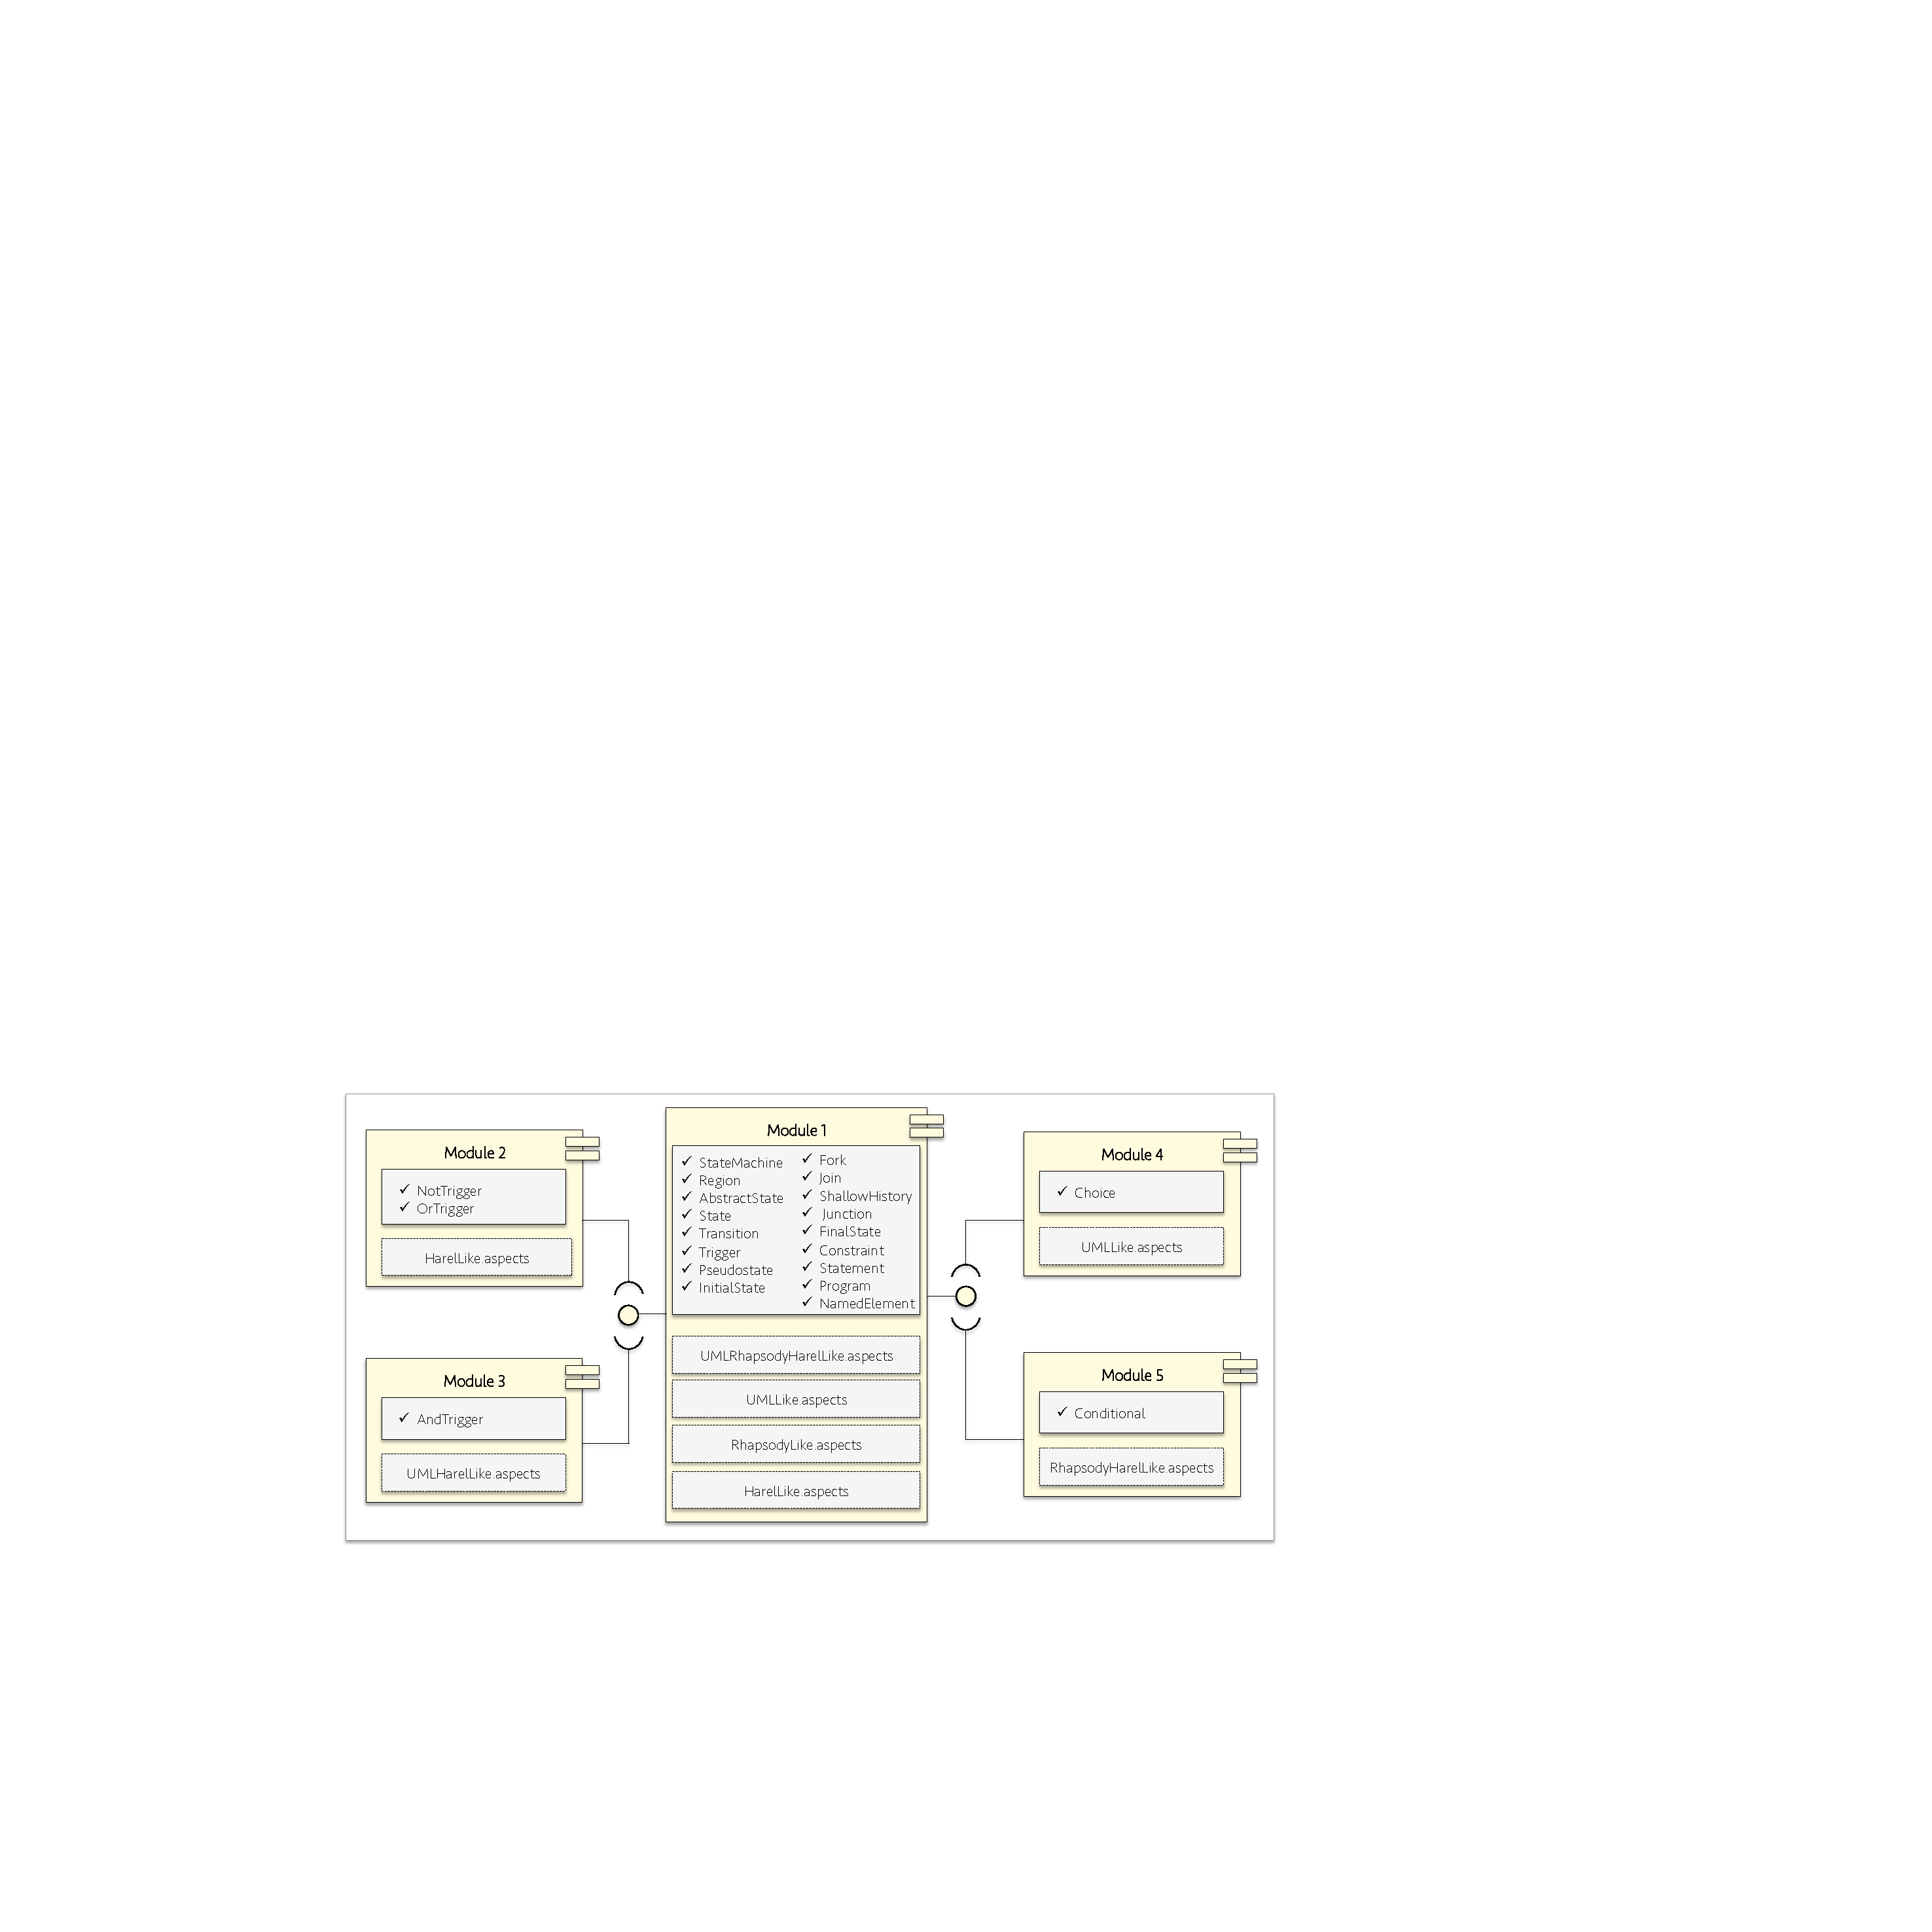
\includegraphics[width=1\linewidth]{images/puzzle-modularization.pdf}
\caption{Results for the state machines case study: extracting language modules}
\label{fig:puzzle-modularization}
\end{figure}

\subsection{Experiment 2: Evaluating \textit{relevance} by identifying potential reuse in the wild}

In order to evaluate the relevance of our approach, we conducted an study on empirical data intended to answer two questions: 1) What is the probability that a DSL has some overlapping with another DSL?; and 2) How big is the average overlapping shared by the existing DSLs? The reminder of this section is dedicated to explain how we obtain the empirical data we use and how we use that data to answer the questions. 
\todo[inline]{que funcion de igualdad has usado aqui? no puedo replicar tu experimento en mi maquina.}
\vspace{-3mm}
\subsubsection{Collecting empirical data:} To collect empirical data, we explored \texttt{GitHub} repositories in search of DSLs that are built on the same technological space that we used in our approach. Namely, metamodels written in Ecore with operational semantics defined as domain-specific actions in Xtend. The objective was to build a realistic data set composed of DSLs developed by diverse development teams. 

As a result of this search, we found \textbf{2424} metamodels (after discarding metamodels with errors). Contrariwise, due to the fact that Kermeta 3 and its implementation in Xtend is a quite recent idea, we found very few data for the semantics part. 

We decided to conduct analysis only in the metamodels thus, the syntactic part of the languages. We consider that such analysis a good insight to know if there is potential reuse.  In the following, we refer to our empirical data as $S$ which is a set of metamodels.

\vspace{-3mm}
\subsubsection{What is the probability that a DSL has some overlapping with another DSL?} To answer this first question, we compute the relative frequency of the event \texttt{E}: \textit{``the metamodel has overlapping with, at least, another metamodel"} in the set $S$. Formally:

\begin{equation}
\begin{split}
P(E) & \approx ~ Relative Frequency (E) = \frac{|S_{E}|}{|S|}\\
& where ~ S_{E} = \{x \in S \mid (\exists y \in S \mid (x \neq y ~ \wedge x \cap y \neq \emptyset )) \}
\end{split}
\end{equation}

Note that computing such probability corresponds to scan the set $S$ in search of occurrences of the event $E$. After doing so, we obtained that that the relative frequency is \textbf{974/2424 = 0.40}.

From a pragmatic point of view, this result means that there are \textbf{40\%} of probabilities that, during the construction of a new DSL, a language designer is replicating at least one metaclass defined in a legacy DSL that is available in \texttt{GitHub}. This probability is quite elevated if we take into account that our comparison operator for metaclases is quite restrictive.

Although this result is quite encouraging, we still wonder how important is the potential reuse. This motivate the following question:

\vspace{-3mm}
\subsubsection{How big is the average overlapping existing among DSLs?} To compute the average of overlapping among the metamodels in the set $S$ we built the matrix illustrated in Figure \ref{fig:matrix-evaluation}. Basically, we performed a pair-wise comparison between the metamodels to obtain the overlapping between all the possible pairs. Then, we compute the average of overlapping that each metamodel has with the other metamodels of the set. To compute that average, we consider only the metamodels where the overlapping is at least 1 metaclass. Finally, we compute the average of these averages.

After executing this experiment, we obtain that the average of overlapping is 3.04. If we analyze the results of questions one and two at the same time, we can conclude that during the construction of the \textbf{40\%} of the new DSLs language designers are replicating, in average, \textbf{3.04} language constructs.
\todo[inline]{porque es tan restrictivo???}
\begin{figure}[h!]
\centering
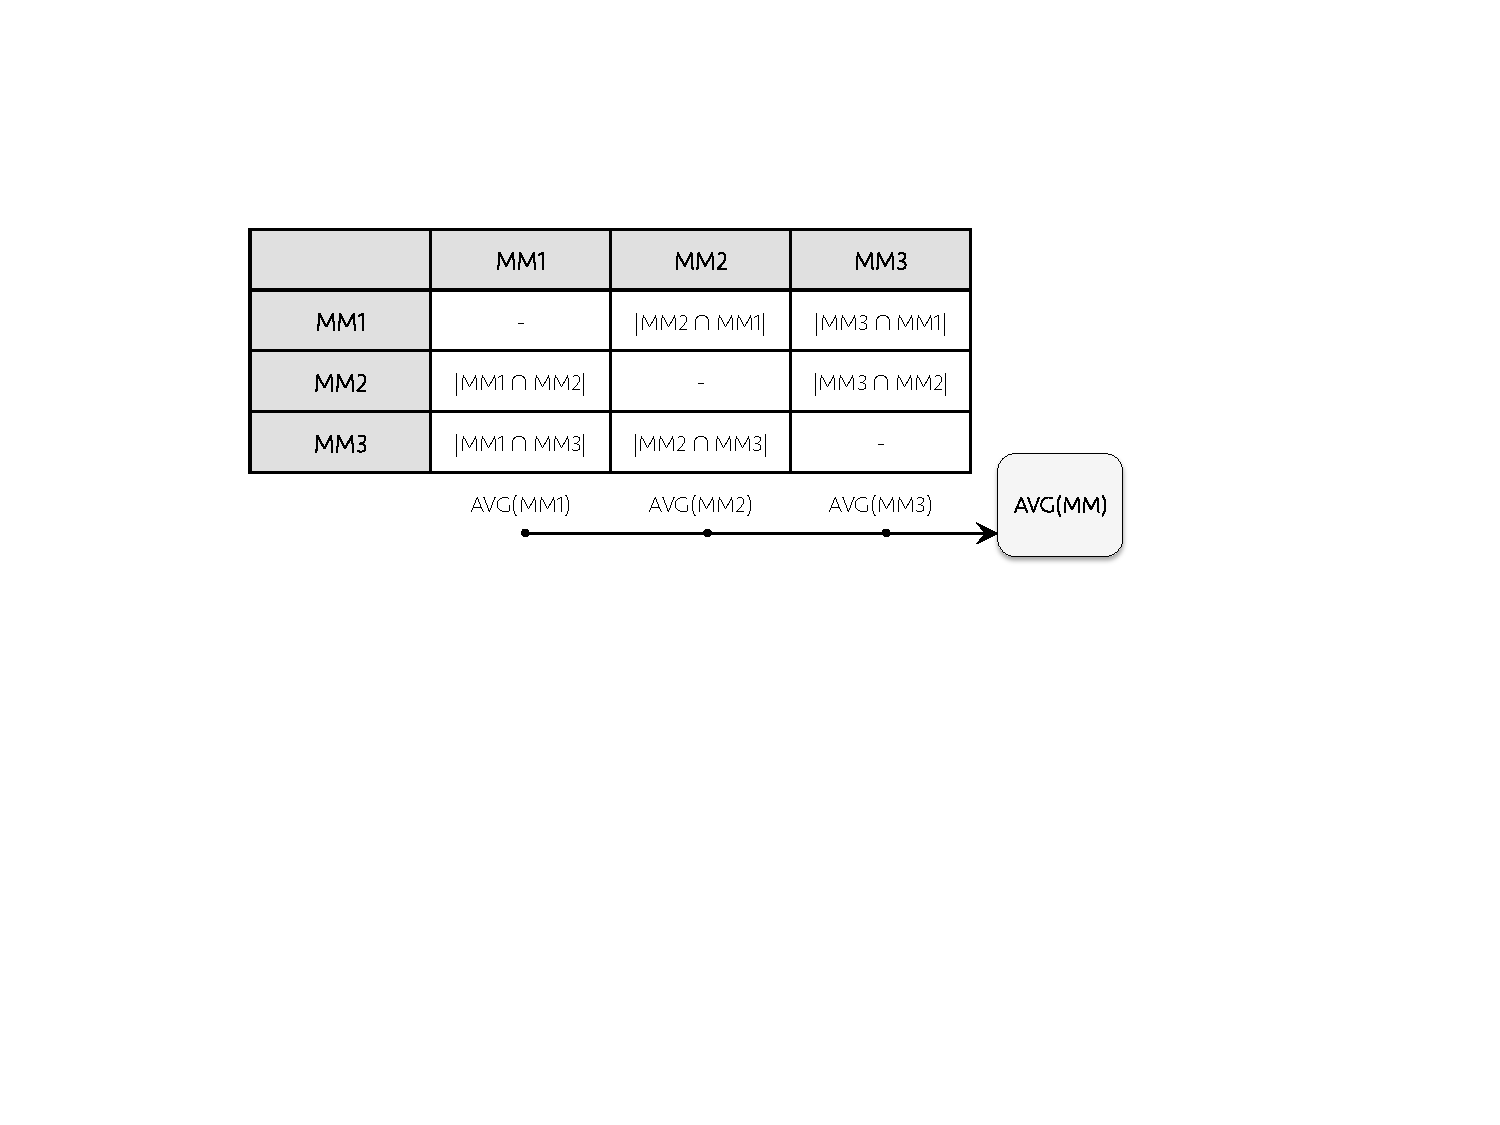
\includegraphics[width=0.75\linewidth]{images/matrix-evaluation.pdf}
\caption{Computing average commonalities}
\label{fig:matrix-evaluation}
\end{figure}

%\vspace{-3mm}
%\subsubsection{Execution platform:} The experiments were conducted using a version of \toolname implemented in Java. Further, \toolname was installed in the Grid5000 Cloud, which is a cluster with more than 5000 cores from were we took XX dual-CPU Dell Blades with Intel Xeon X3470 CPUs running at 2.93GHz, with 16 threads per CPU, and CentOS v6. Each dual-CPU Dell Blade has 36GB of RAM. 


%\begin{table*}[htbp]
%  \centering
% \scalebox{0.8}{
%\begin{tabular}{|p{0.2\textwidth}|p{0.3\textwidth}p{0.1\textwidth}p{0.4\textwidth}|}
%\hline
%\multicolumn{4}{|c|}{\textbf{Hypotheses of Experiment 1}} \\ \hline
%\textbf{Null Hypothesis ($H_0$)} & \multicolumn{ 3}{|p{0.8\textwidth}|}{\toolname is capable of detecting %commonalities in the case study that motivated this research.} \\ \hline
%\textbf{Alt. Hypothesis ($H_1$)} & \multicolumn{ 3}{|p{0.8\textwidth}|}{
%\toolname is not capable of detecting commonalities in the case study that motivated this research.} \\ %\hline
%\textbf{Dependent variable} & \multicolumn{ 3}{|p{0.8\textwidth}|}{The set of ecores representing our %languages. }\\ \hline
%\textbf{Blocking variables} & \multicolumn{ 3}{|p{0.8\textwidth}|}{The most sold phones and the market %share indexes. }\\ \hline
%\textbf{Model used as input} & \multicolumn{ 3}{|p{0.8\textwidth}|}{\textit{models in %\url{urlhacialosmodelos}} }
%\\
%\hline \hline


%\multicolumn{4}{|c|}{\textbf{Hypotheses of Experiment 2}} \\ \hline
%\textbf{Null Hypothesis ($H_0$)} & \multicolumn{ 3}{|p{0.8\textwidth}|}{The use of \toolname 
%will not result in a higher market-share impact metric than selecting the most commonly sold 
%phones, for a given maximum budget.} \\ \hline
%\textbf{Alt. Hypothesis ($H_1$)} & \multicolumn{ 3}{|p{0.8\textwidth}|}{The use of \toolname 
%will result in a higher market-share impact metric than selecting the most commonly sold 
%phones, for a given maximum budget.}\\ \hline
%\textbf{Model used as input} & \multicolumn{ 3}{|p{0.8\textwidth}|}{\textit{Android feature model presented %in Figure \ref{fig:featureModel}} }\\ 
%\hline
%% @J - Do you mean independent?! My understanding is that a blocking variable is a grouping variable...
%\textbf{Blocking variables} & \multicolumn{ 3}{|p{0.8\textwidth}|}{The most sold phones, market share %indexes and the maximum cost allowed set to 600\$. }\\ \hline
%\textbf{Model used as input} & \multicolumn{ 3}{|p{0.8\textwidth}|}{\textit{Android feature model presented in Figure \ref{fig:featureModel}} }\\
%\hline \hline

%\multicolumn{4}{|c|}{\textbf{Constants}} \\ \hline
%\textbf{CSP solver} & \multicolumn{ 3}{|p{0.8\textwidth}|}{\textit{ChocoSolver v2} } \\ \hline
%\textbf{Heuristic for variable selection in the CSP solver} & \multicolumn{ 3}{|p{0.8\textwidth}|}{\textit{Default}}\\
%\hline 

%\hline 
%\end{tabular}%
%}
%\caption{Hypotheses and design of experiments.}
%  \label{tab:Exp1aDesign}
%\end{table*}
%\todo{poner la tabla para con los datos de los experimentos que vamos a ejecutar/hemos ejecutado. Intenta pensar cuales pueden ser las conclusiones que quieres extraer. Yo propongo 3 abajo.}

%Table \ref{tab:Exp1aDesign} shows the hypothesis of the experiments executed to validate our 
%approach. To make the experiments reproducible, a number of fixed assumptions are made, such as homogeneous feature costs. ChocoSolver 
%\footnote{\url{http://www.emn.fr/z-info/choco-solver/}}, with it's default heuristic, is 
%used as the CSP solver for extracting software products from the feature model presented 
%in Figure \ref{fig:featureModel}

%\textbf{Technological space and experimental platform:} Currently, there are diverse techniques available for the implementation of syntax and semantics of DSLs \cite{Mernik:2005b}. Language designers can, for example, choose between using context-free grammars or metamodels as specification formalism for syntax. Similarly, there are at least three methods for expressing semantics: operationally, denotationally, and axiomatically \cite{Mosses:2001}. In this paper we are interested on DSLs which syntax is specified by means of metamodels and semantics is specified operationally as a set methods (a.k.a, \textit{domain-specific actions} \cite{Combemale:2013}). Each language construct is specified by means a metaclass and the relationship between language constructs are specified as references between metaclasses. In turn, domain-specific actions are specified as java-like methods that are allocated in each metaclass.
